\subsubsection{Registration}
The registration service is used to register a new user so that they may be able to store they're preferences. To register you need to click on the "signup" button on the landing page. After you click the button a popup form will appear as show in the picture below. You need to fill out the form with a valid email address and then click the register button. This will send an email with a randomly generated password which you need to login in. The login procedure is explain later in the text. \\[0.5cm]
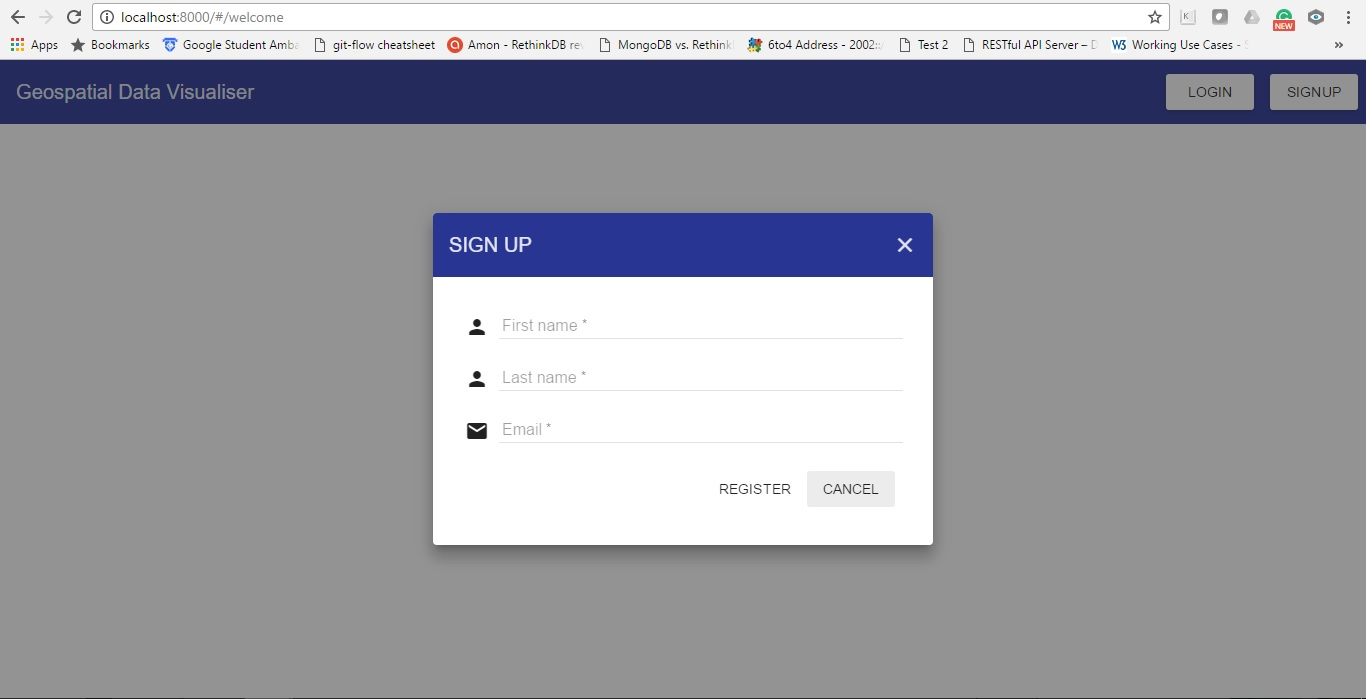
\includegraphics[width=\textwidth]{registerFunction} \\[0.5cm]
\subsubsection{Login}
This function is used to login in so that you may use the site. \\[0.5cm]
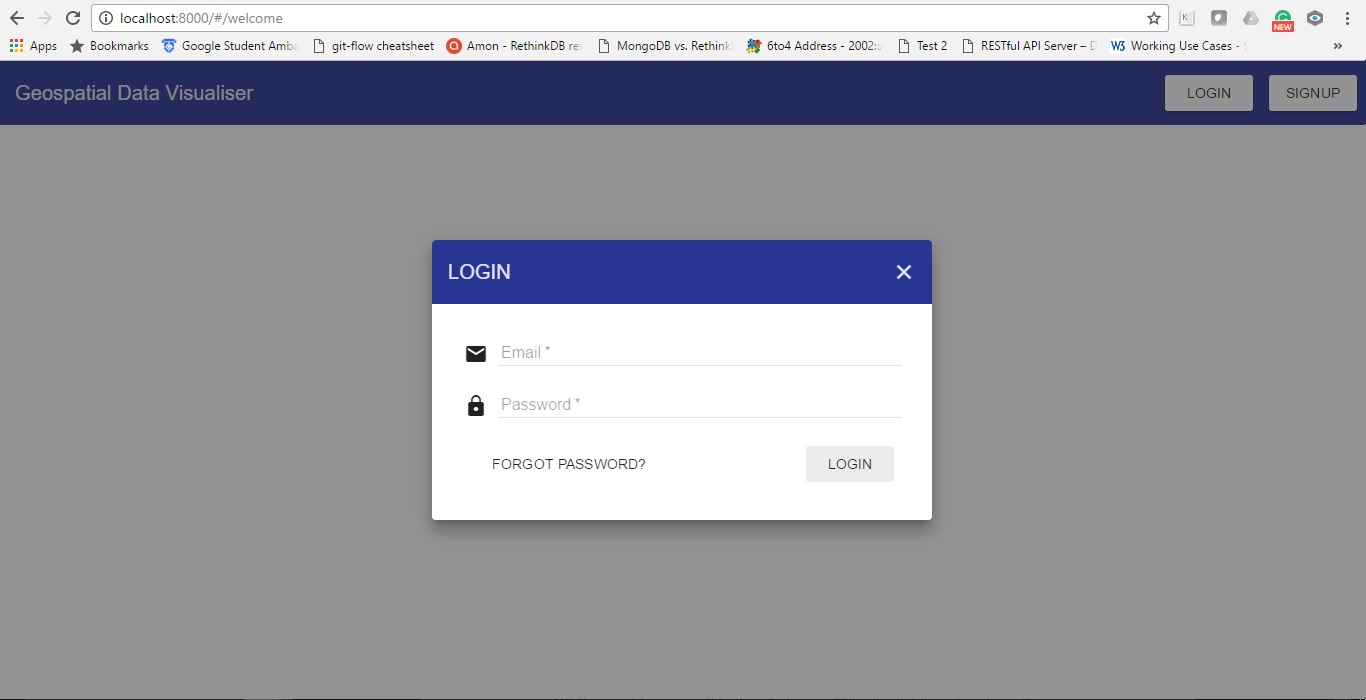
\includegraphics[width=\textwidth]{loginFunction} \\[0.5cm]
To login you need to click the "login" button to the left of the "signup" button on the landing page. Once you click the button a popup form will appear shown in the picture above. You need to fill out the form with the email you used to register and the password you received through email. After you fill out the form click the login in button to proceed.
\subsubsection{Location Search}
The search service, is used to search and load any place in the world. As shown in the figure below, you need to click in the search box and start typing the name of the place you are searching for. \\[0.5cm]
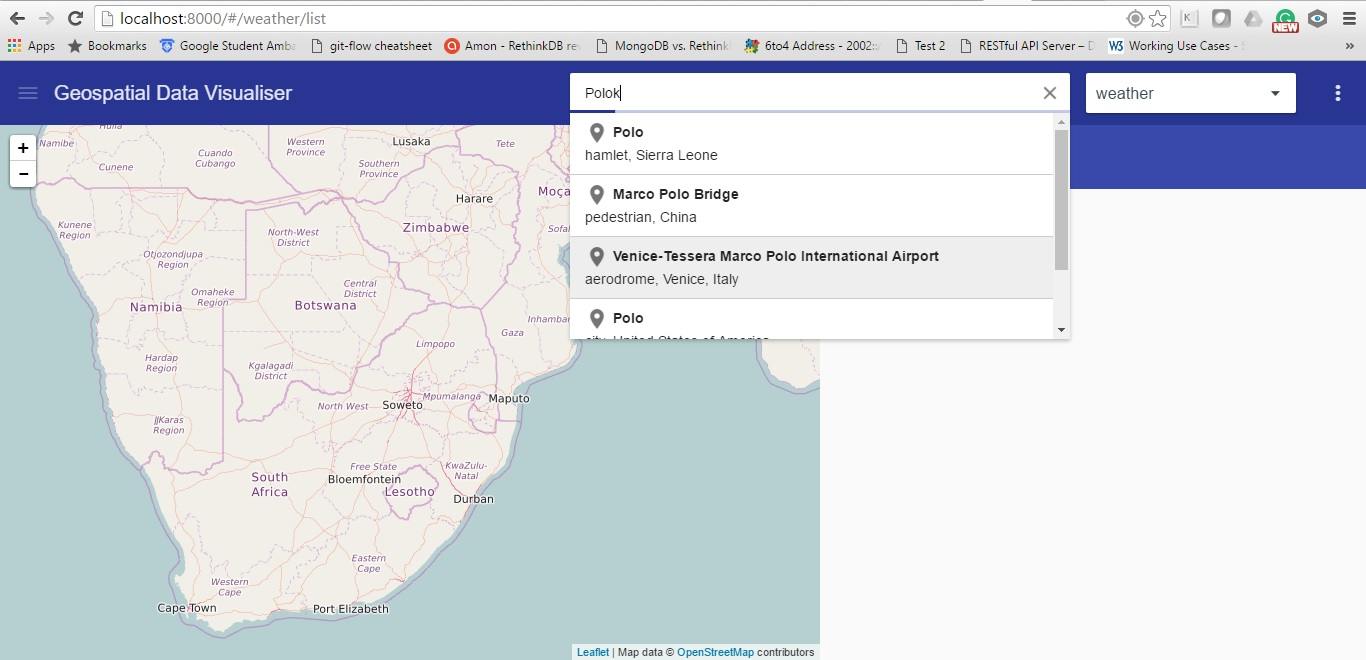
\includegraphics[width=\textwidth]{searchFunction} \\[0.5cm]
While searching a possible list of places will be loaded in a dropdown list as shown in the figure above. Once you have found the place you are looking for, use your mouse to point to the name of the place and click on that name, which will then activate a process of reloading the map to the place you have selected, like the figure shown below. A marker will be placed to show the location you queried. \\[0.5cm]
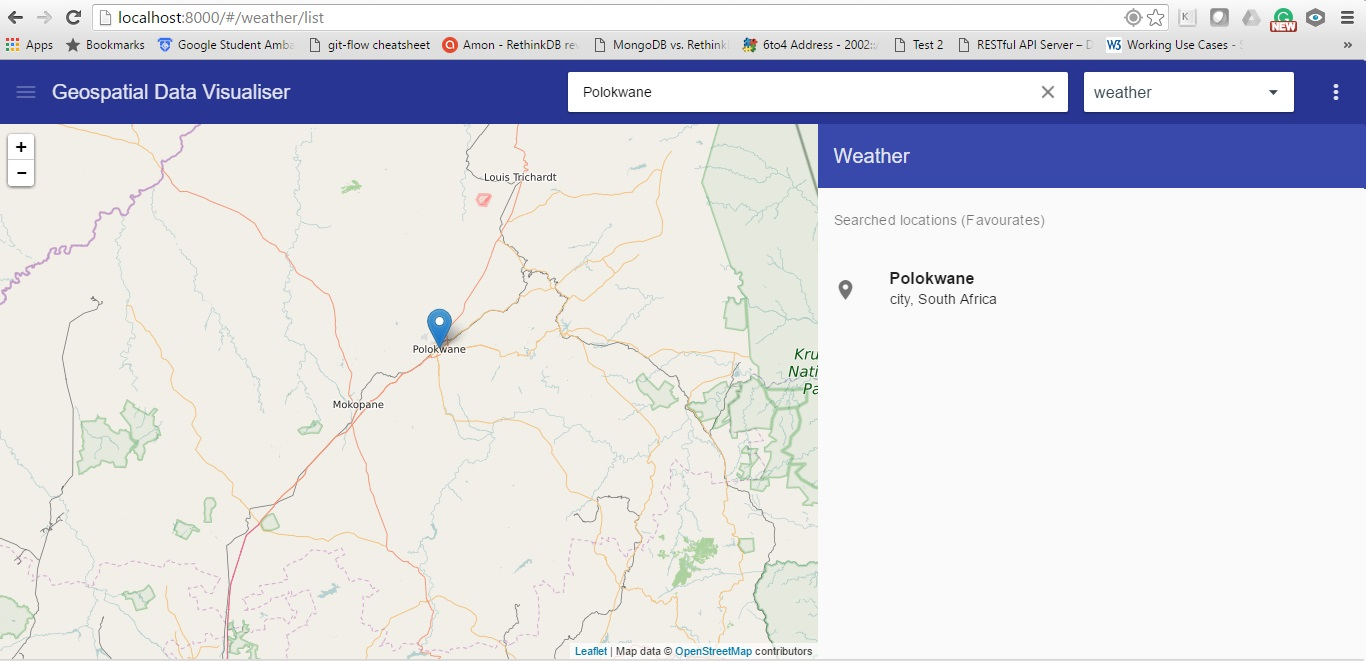
\includegraphics[width=\textwidth]{searchResult} \\[0.5cm]
The search feature is also linked to other functions of the site. When the weather center is currently active, the location name will be added to the listed of locations you have already searched for as shown above. These features will be explained in more detail in sections about the respective features.
\subsubsection{Disaster Center}
To navigate to the disaster center. Click on the "Center navigation" and move you mouse cursor over the "disasters" button on the dropdown list and click. Shown in the the figure below. \\[0.5cm]
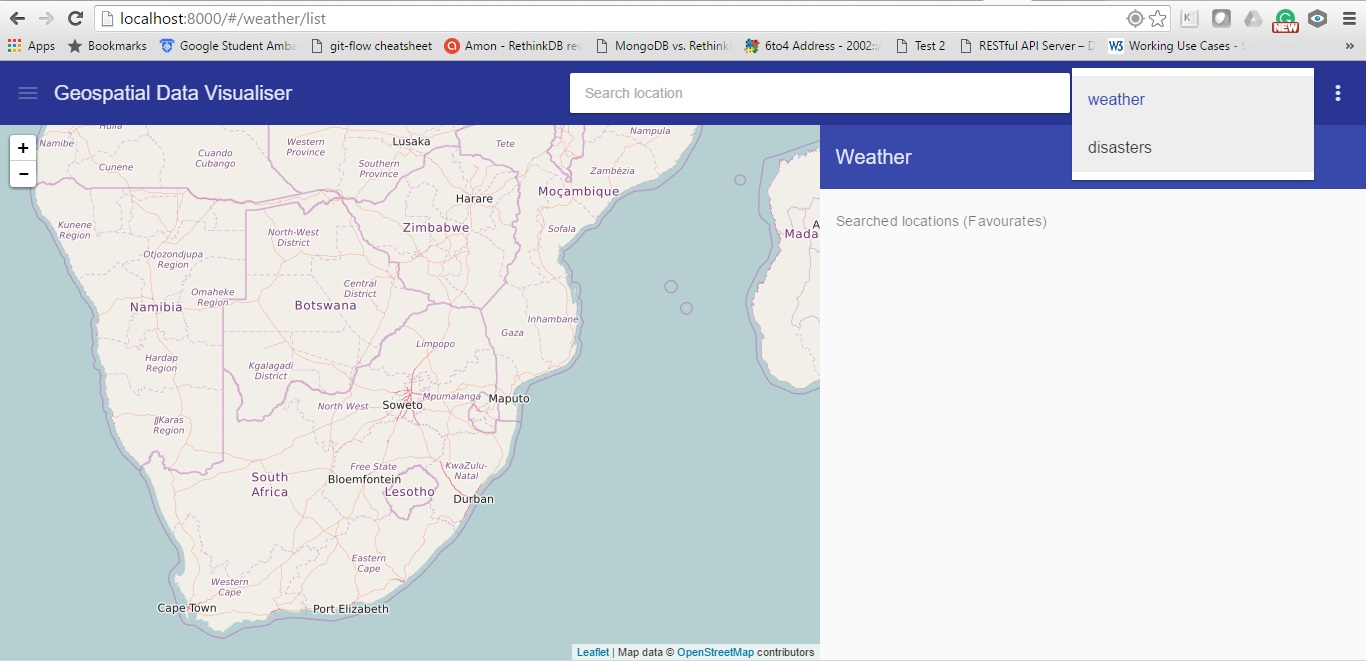
\includegraphics[width=\textwidth]{disaster1} \\[0.5cm]
Once you have loaded the disaster center, you will land on the page shown in the figure below below. The numbers on the figure show the features currently available in the disaster center. \\[0.5cm]
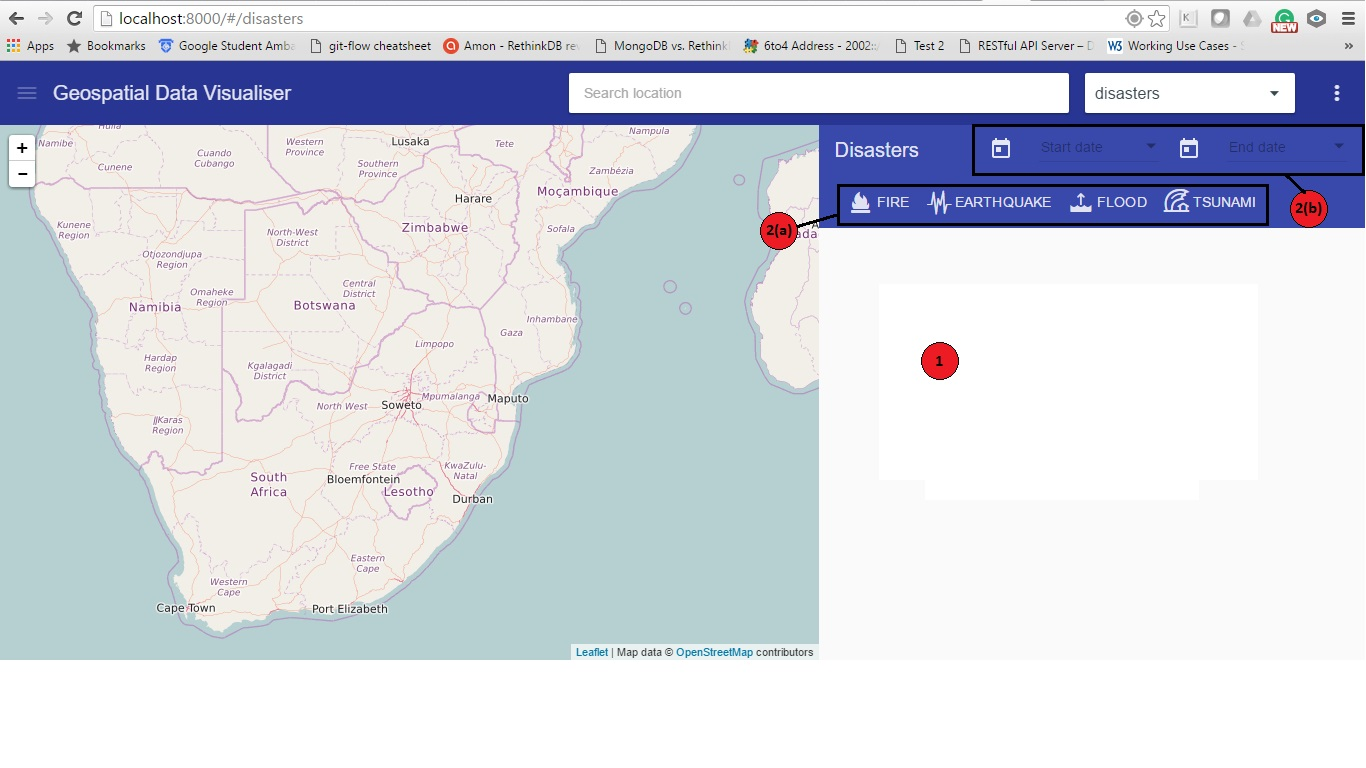
\includegraphics[width=\textwidth]{disaster2} \\[0.5cm]
	\begin{enumerate}
		\item \textbf{List of disasters} : This part of the center will show the list of disasters that are currently displayed on the map area. It will allow the user to load more information about each disaster displayed on the map area. For example, if a user decides to show earthquakes as shown in the figure below. The earthquakes or any disaster for that matter will be loaded on to the map area. The blue icons show a number of disasters clustered in a specific range of area the blue icon lays over. Each individual disaster then has its own type of icon. Earthquakes shown by yellow icons, fires by red etc. As you may see from the figure below, only the individual disasters are shown on the list. \\[0.5cm]
		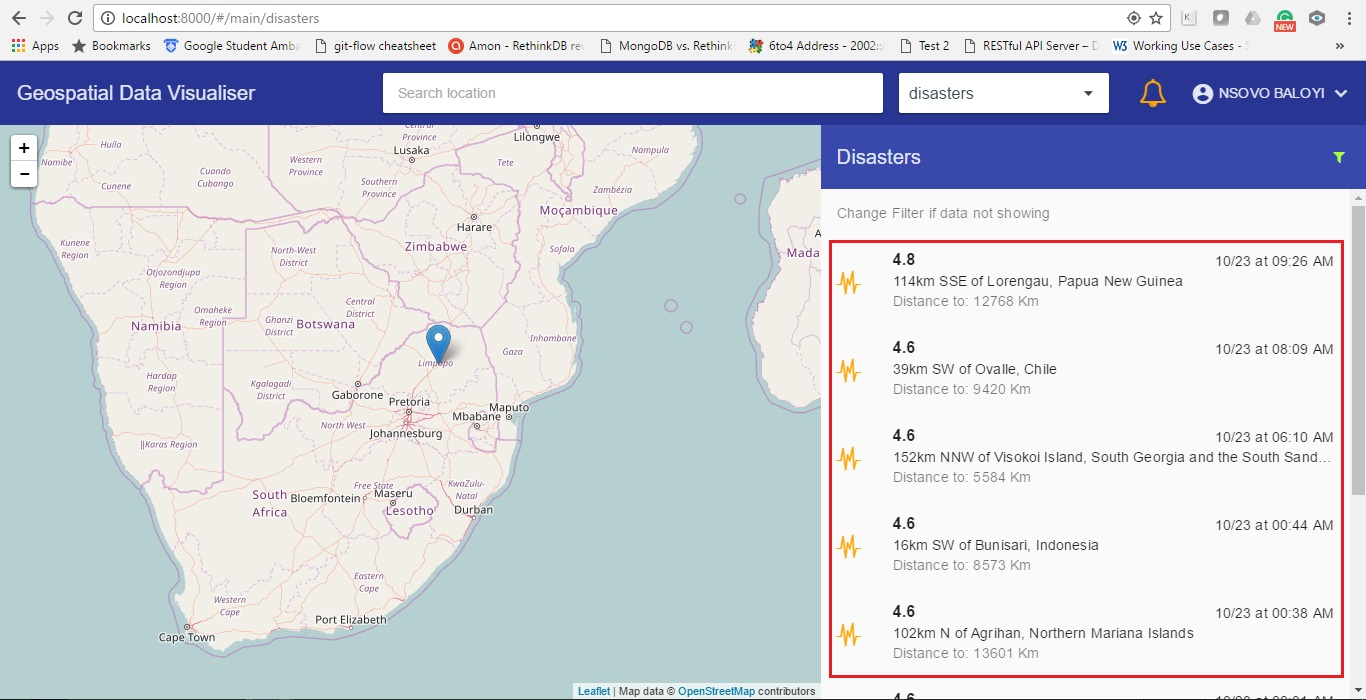
\includegraphics[width=\textwidth]{disaster3} \\[0.5cm]
		By moving the map to another location you then refresh the list by loading the disaster currently visible on the map area.
		\item \textbf{Notification Feature} : This part of the center will notify the user of any new active disasters or updated disasters. A red circle with the number of new disasters will popup, as show in the picture below, to notify the user of active disasters.\\[0.5cm]
		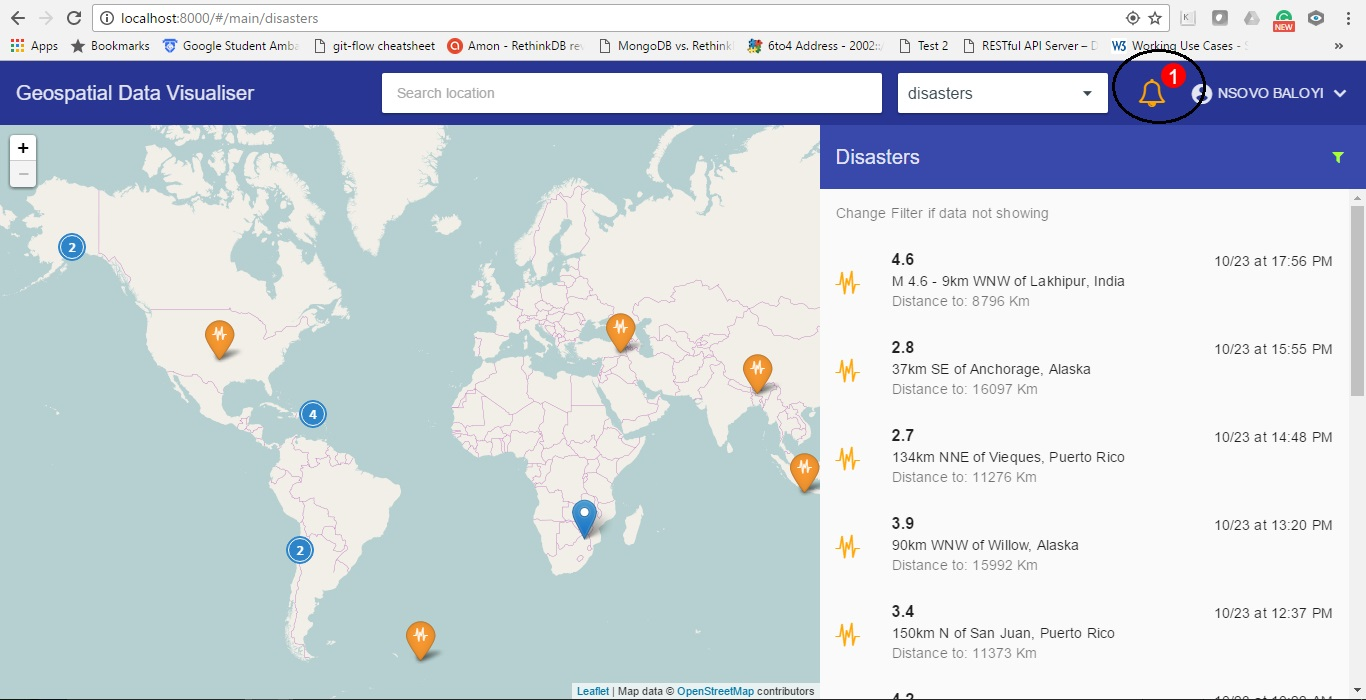
\includegraphics[width=\textwidth]{disaster6}\\[0.5cm]
		\item \textbf{Query Features} : 
		This section describes how the query features may be used.\\[0.5cm]
		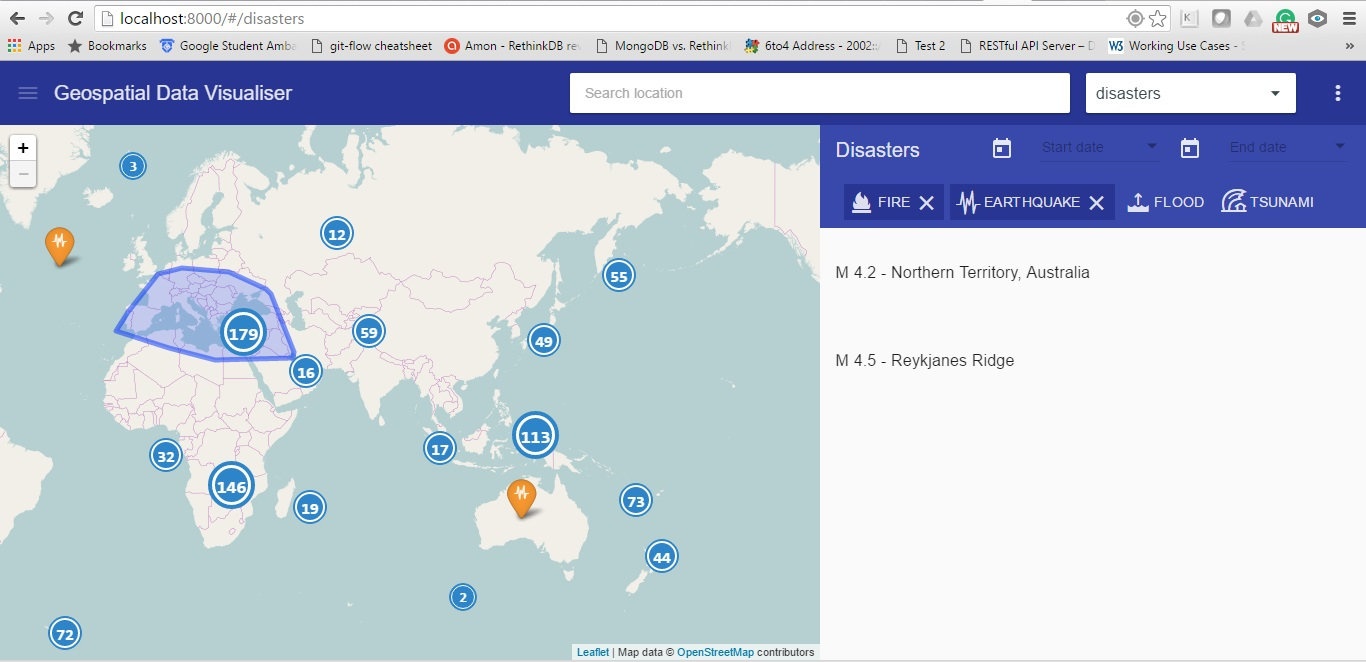
\includegraphics[width=\textwidth]{disaster4} \\[0.5cm]		
		\begin{enumerate}
		\item \textbf{Filter Button}: To filter the disaster data click the button labelled 2(a) in the image above. This will open a form which the user may change to suit their preferences. 
		\item \textbf{Filter Form}: The form allows you to filter disasters by time and by distance as well as disaster features for example magnitude in the case of earthquakes.
		\end{enumerate}
		As stated above, once a query is performed, the disasters are loaded onto the map area. The blue icons show the number of disasters clustered in a range. When you click one of these blue icons, the system perform a zoom service to the location of that icon. This then reveals more blue icons or disasters hidden by the clustering feature. By clicking another blue icon another zoom service is performed again etc.
	\end{enumerate}
\subsubsection{Weather Center}
Like the Disaster center to navigate to the disaster center. Click on the "Center navigation" and move you mouse cursor over the "weather" button on the dropdown list and click. Shown in the the figure below. \\[0.5cm]
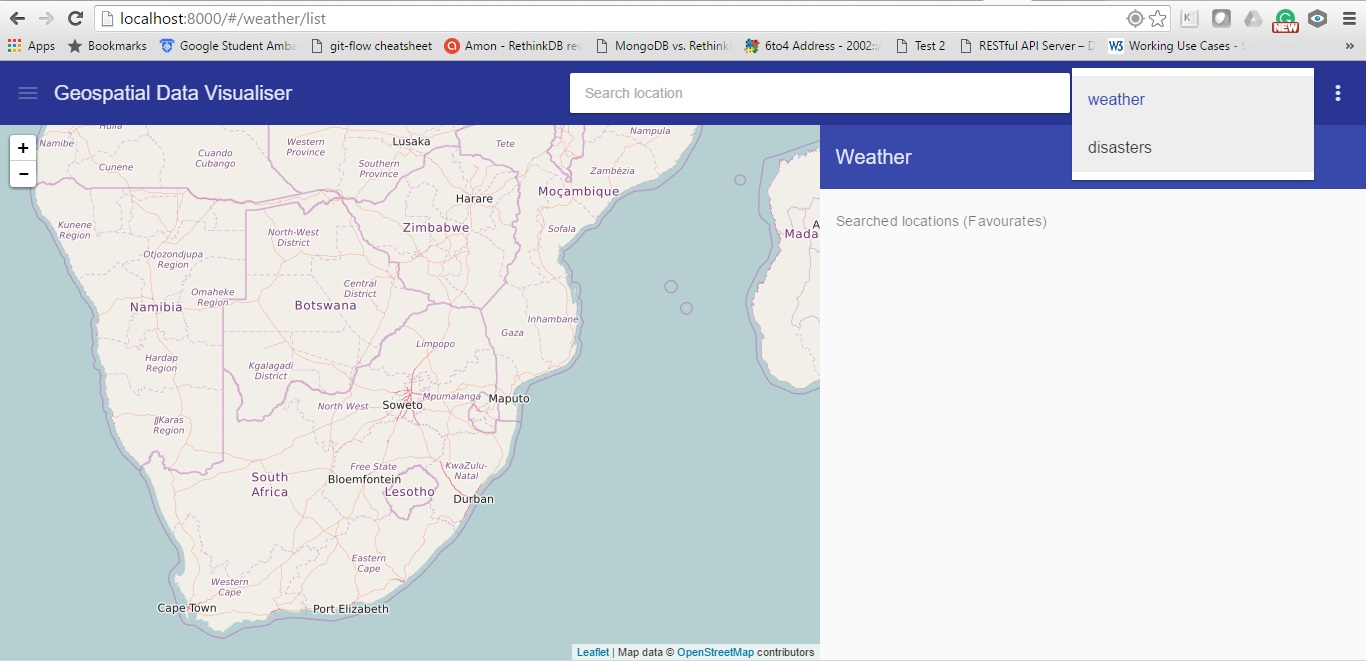
\includegraphics[width=\textwidth]{disaster1} \\[0.5cm]
Once you have loaded the weather center, you will land on the page shown in the figure below below. The numbers on the figure show the features currently available in the disaster center. \\[0.5cm]
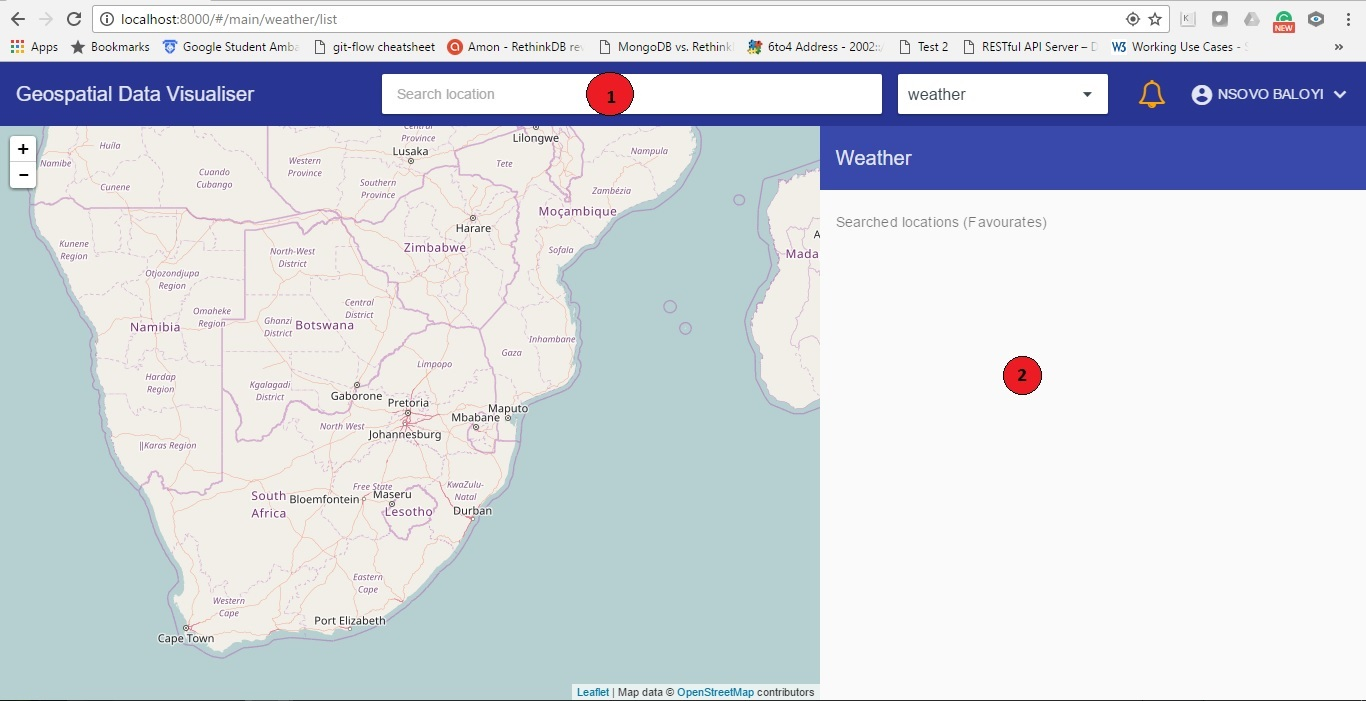
\includegraphics[width=\textwidth]{weather1} \\[0.5cm]
	\begin{enumerate}
		\item \textbf{Search} : The search feature works hand in hand with the weather center. You are required to first search for a location by using the search feature as explained in 2.2.3
		\item \textbf{Weather List}
		Once you have search for a location it is added to locations on the weather list section as show in the figure below. \\[0.5cm]
		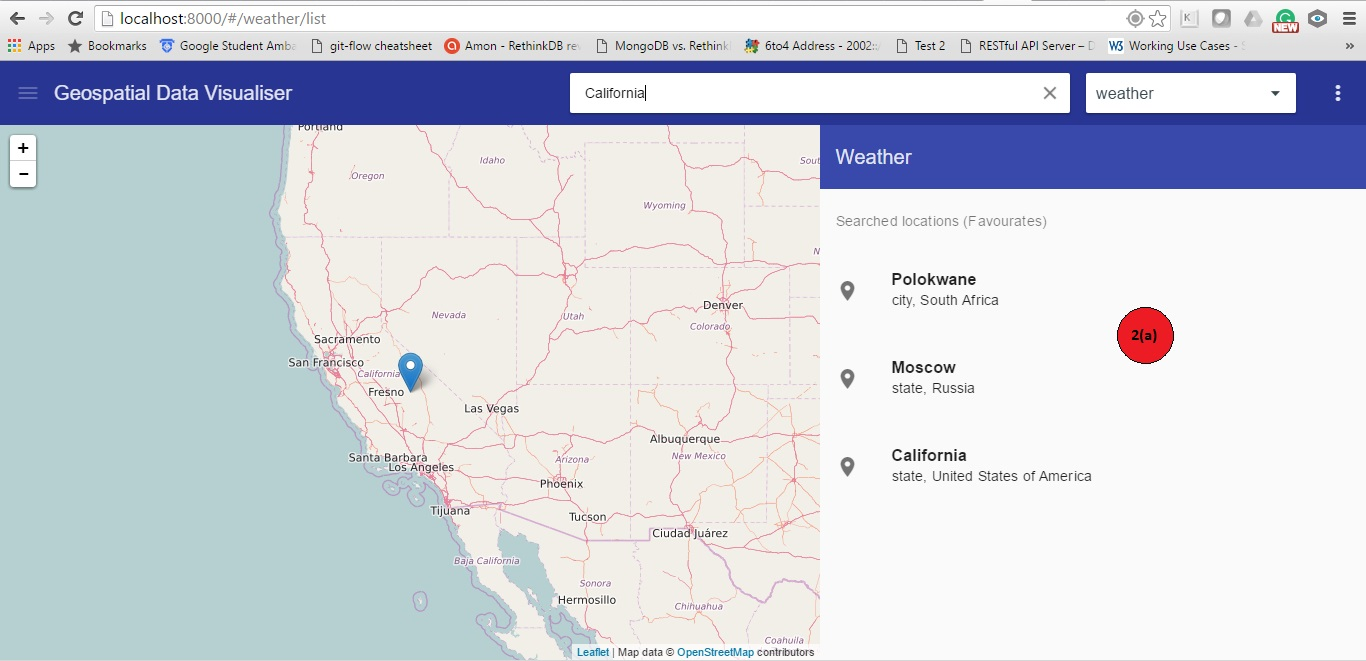
\includegraphics[width=\textwidth]{weather2} \\[0.5cm]
		\begin{enumerate}
		\item \textbf{List of locations}: The figure above shows the locations loaded after searching. To load the current weather of a location on the list. You need to use your mouse and hover over on of the items on the list and click. 
		\item \textbf{Selected location}: Once a location is selected from the list of locations, more details about that locations weather is loaded as show in the figure below. To navigate back to the list of locations, you must click the back button as shown by the red circle in the figure below. \\[0.2cm]
		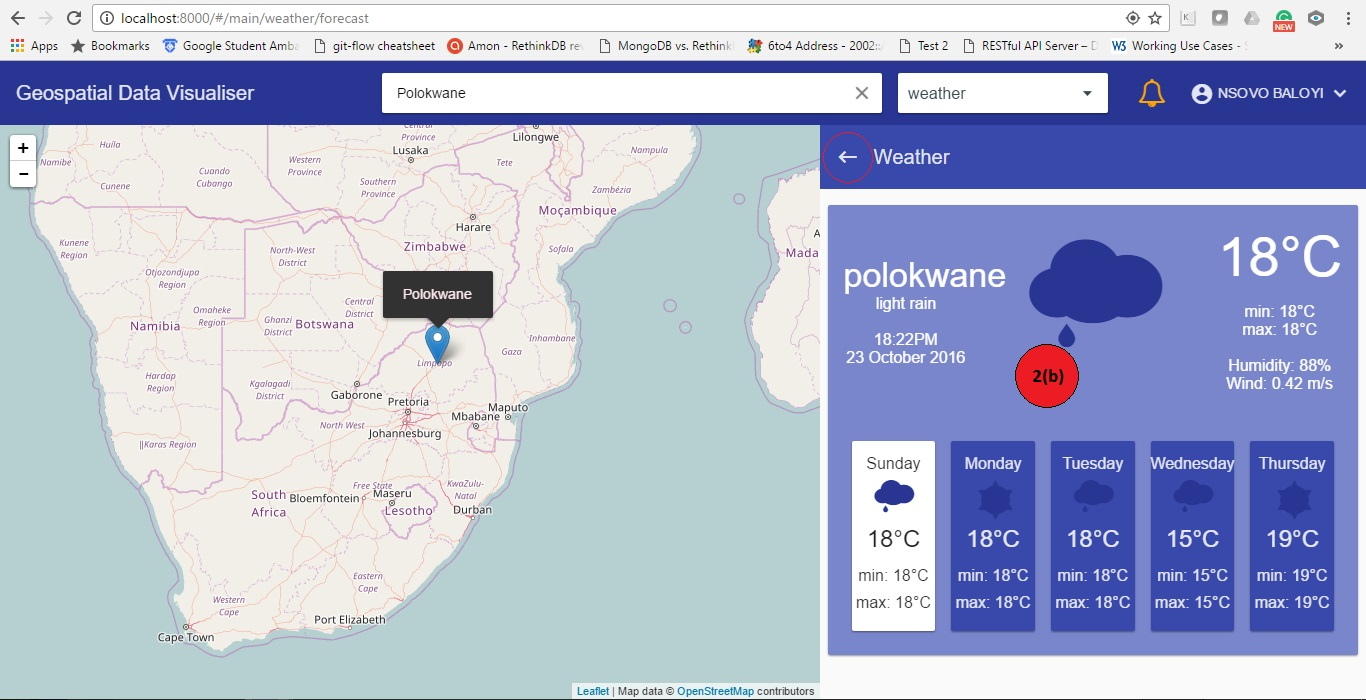
\includegraphics[width=\textwidth]{weather3} \\[0.5cm]
		\end{enumerate}
	\end{enumerate}
\subsubsection{Map Features}
The features that are listed below will be are part of the map service provided by the system, these include:
\begin{enumerate}
\item \textbf{Zoom feature}:\\
Allows you to zoom the map in and out by clicking the zoom button mentioned before.

\item \textbf{On map area click feature}\\
This feature zooms the map when you click an icon or over the mouse of a location name on the weather center.
\item \textbf{On map click and drag}\\
Allows you to click and drag the map to a point you would like to see.
\end{enumerate}

